%%%%%%%%%%%%%%%%%%%%%%%%%%%%%%%%%%%%%%%%%%%%%%%%%%%%%%%%%%%%%%%%%%%%%%%%%%
 %																		%
 %	Plantilla Latex para presentación del proyecto de curso				%
 %	Programación de Aplicaciones para Internet y la Nube					%
 %																		%
 %	Creada por: Duván Pardo, Wilson López								%
 %																		%
 %	Versión: 0.1															%
 %	Dapardoc@gmail.com ; Wilrilo@gmail.com								%
 %																		% 
 %	Se requieren los archivos plantilla.bbl y							% 
 %	El directorio Imagenes que contiene: CECAD,DC, Elementos y RITA		%  
 %																		%
%%%%%%%%%%%%%%%%%%%%%%%%%%%%%%%%%%%%%%%%%%%%%%%%%%%%%%%%%%%%%%%%%%%%%%%%%%

\documentclass[10pt]{article}   			% Describe el tipo de documento, y el tamaño de la letra del texto

\usepackage[utf8]{inputenc}				% Define codificación para que permita caracteres latinos (acentos)
\usepackage[spanish,activeacute]{babel} 	% Paquete para poder escribir con tildes y otros caracteres especiales

\usepackage{vmargin}						% Código para margenes y formato de página
\setpapersize{A4}
\setmargins	{2.2cm}     					% margen izquierdo
			{1 cm}                 		% margen superior
			{16.5cm}               		% anchura del texto
			{23.42cm}             		% altura del texto
			{20pt}                		% altura de los encabezados
			{1.2cm}               		% espacio entre el texto y los encabezados
			{0pt}                		% altura del pie de página
			{2cm}                 		% espacio entre el texto y el pie de página

\usepackage{amsmath}						% paquete para expresiones matemáticas
\usepackage{amsfonts}					% paquete para escritura de ecuaciones 
\usepackage{amssymb}						% paquete para caracteres especiales para ecuaciones 

\usepackage{fancyhdr}					% Temas para encabezado y pie de pagina
\usepackage{fancyvrb}
\pagestyle{fancy} 

\pagenumbering{arabic} 					% Numeración de paginas {arabic roman}
\usepackage{hyperref}					% Para hipervinculos
\usepackage{graphicx}					% Para incluir imágenes
\usepackage{float}
\usepackage{caption}						% Descripciones de las figuras
\usepackage{subcaption}					% Descripción varias imagenes en usa sola figura
\graphicspath{ {Imagenes/} }				% Directorio de imágenes esta capeta va donde esta el archivo tex


\usepackage{color, colortbl}				% Colores para tablas
\usepackage{listings}					% Para el código Fuente
\usepackage{xcolor}						% para color en codigos o listrings
\definecolor{limegreen}{RGB}{50,100,50}	% Definición de colores ejemplo verde en RGB
\definecolor{Red}{RGB}{220,120,120}		% se definen colores para la tabla en el cronograma pueden ser RGB 0-255 o rgb 0-1 cada componente
\definecolor{LightCyan}{rgb}{0.88,1,1}
\definecolor{azul}{RGB}{120,120,210}


\lstset{numbers=left, numberstyle=\tiny, stepnumber=2, numbersep=5pt}

%Aquí inicia el documento.
\begin{document}
	% Se define el Encabezado
	%clhead[]{Proyecto}
	\lhead[]{Programación de Aplicaciones para Internet y la Nube}
	\rhead[]{\textbf{2016-I}}
	\renewcommand{\headrulewidth}{0.5pt}

	\thispagestyle{empty}						% La primera página no lleva estilo (sin encabezado)
	\begin{center}
		\large {Programación de Aplicaciones para Internet y la Nube
			\hspace{5 cm}\textbf{2016-I}}
		\bigskip  
		\textbf{
				\LARGE{\\TALLER 7}}\\								% Nombre del proyecto
	\end{center}	
	\begin{flushright}	
		\bigskip	
		Nombre del Estudiante: \textbf{Duván Pardo, Wilson López}			% Nombre del estudiante
	\end{flushright} 
	
\section{INTRODUCCIÓN}	

Los contenedores Docker envuelven una pieza de software en un sistema de archivos completo que contiene todo lo que necesita para funcionar: código, runtime, herramientas del sistema, bibliotecas del sistema - cualquier cosa que usted puede instalar en un servidor. Esto garantiza que siempre se ejecutará la misma, independientemente del entorno en el que se está ejecutando.\\


\textbf{¿Cómo se diferencia de las máquinas virtuales?}\\

Los contenedores tienen aislamiento de asignación de recursos y beneficios similares a los de las máquinas virtuales, pero un enfoque arquitectónico diferente que les permite ser mucho más portátil y eficiente. (tomado de \href{https://www.docker.com/what-docker}{Docker})\\



\textbf{Máquinas virtuales}\\

Cada máquina virtual incluye la aplicación, los binarios y librerías necesarias y todo un sistema operativo invitado - los cuales pueden ser decenas de GB de tamaño. 
		\begin{figure}[ht]
			\centering
			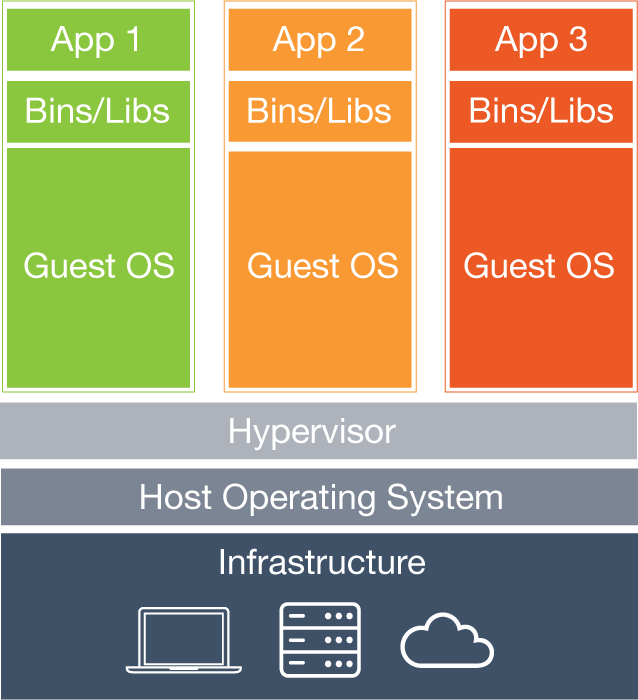
\includegraphics[scale=0.3]{mvir}   
			\caption{Diagrama de la máquina virtual(tomado de \href{https://www.docker.com/sites/default/files/what-is-docker-diagram.png}{https://www.docker.com/sites/default/files/what-is-docker-diagram.png})  } 
		\end{figure}
		
\textbf{Contenedores}

Los contenedores incluyen la aplicación y todas sus dependencias, pero comparten el núcleo con otros contenedores. Corren como un proceso aislado en el espacio de usuario en el sistema operativo anfitrión. Asimismo, no están vinculados a ninguna infraestructura específica - los contenedores Docker se ejecutan en cualquier ordenador, en cualquier infraestructura y en cualquier nube.	(tomado de \href{https://www.docker.com/what-docker}{Docker})
\newpage
	\begin{figure}[ht]
		\centering
		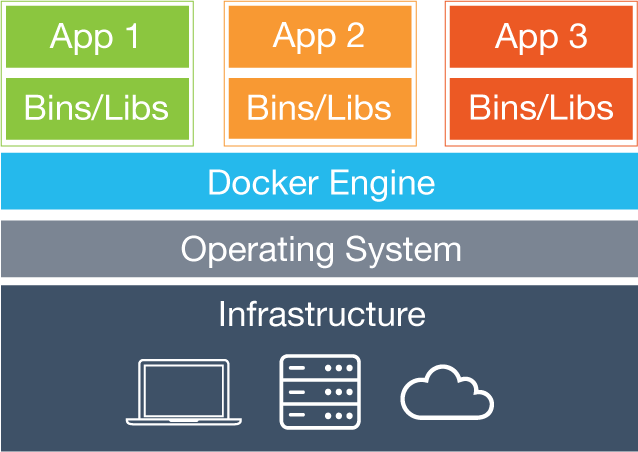
\includegraphics[scale=0.3]{contenedores}   
		\caption{Diagrama de los contenedores(tomado de \href{https://www.docker.com/sites/default/files/what-is-vm-diagram.png}{https://www.docker.com/sites/default/files/what-is-vm-diagram.png})} 
	\end{figure}
	

	
\section{OBJETIVO}
Realizar el despliegue de aplicaciones sencillas mediante la tecnología Docker sobre el sistema operativo Linux Ubuntu Server.
\section{ACTIVIDADES}	

\begin{enumerate}


\item  Verificar la correcta instalación del servicio Docker ejecutando el comando: \\
\begin{center}
	\texttt{sudo service docker status}
\end{center}
\begin{figure}[ht]
	\centering
	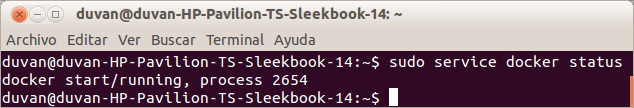
\includegraphics[scale=0.5]{1}   
	\caption{Correcta instalación del servicio Docker } 
\end{figure}

\item 	En este taller se va a utilizar un archivo denominado Dockerfile (similar al Vagrafile) que establece el conjunto de pasos para desplegar una imagen Docker. Crear un directorio, entrar a ese directorio y crear un archivo llamado “\texttt{\href{https://github.com/wilrilo/talleres/blob/master/file/taller7/files/docker/Dockerfile}{Dockerfile}}”.

\begin{figure}[ht]
	\centering
	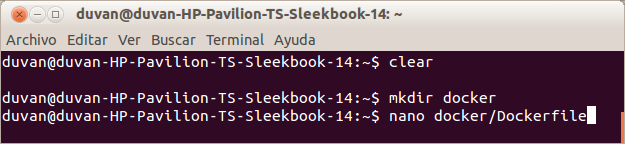
\includegraphics[scale=0.5]{2}   
	\caption{Creación archivo \textit{Dockerfile}} 
\end{figure}


\item Ingresar el siguiente contenido en el archivo “\texttt{\href{https://github.com/wilrilo/talleres/blob/master/file/taller7/files/docker/Dockerfile}{Dockerfile}}”:
\begin{small}
	\begin{lstlisting}[frame=single]	
FROM ubuntu:trusty

RUN sudo apt-get update && sudo apt-get -y install cowsay fortune
	\end{lstlisting}
\end{small}
\newpage
Existen distintas fuentes para cada imagen (para el comando FROM), para realizar una búsqueda es posible por medio del comando :
%%
\begin{figure}[H]
	\centering
	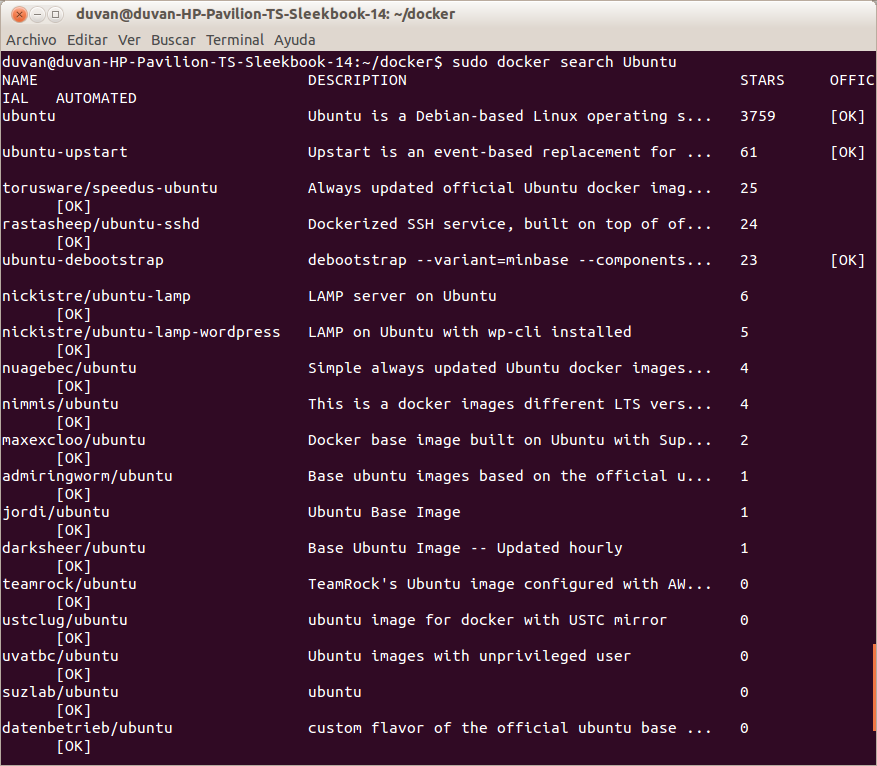
\includegraphics[scale=0.3]{31}   
	\caption{Búsqueda con el comando \texttt{search} } 
\end{figure}

\item Construir una nueva imagen a partir del “\texttt{\href{https://github.com/wilrilo/talleres/blob/master/file/taller7/files/docker/Dockerfile}{Dockerfile}}”

\begin{center}
	\texttt{sudo docker build -t test/dockerfile-example}
\end{center}
\begin{figure}[ht]
	\centering
	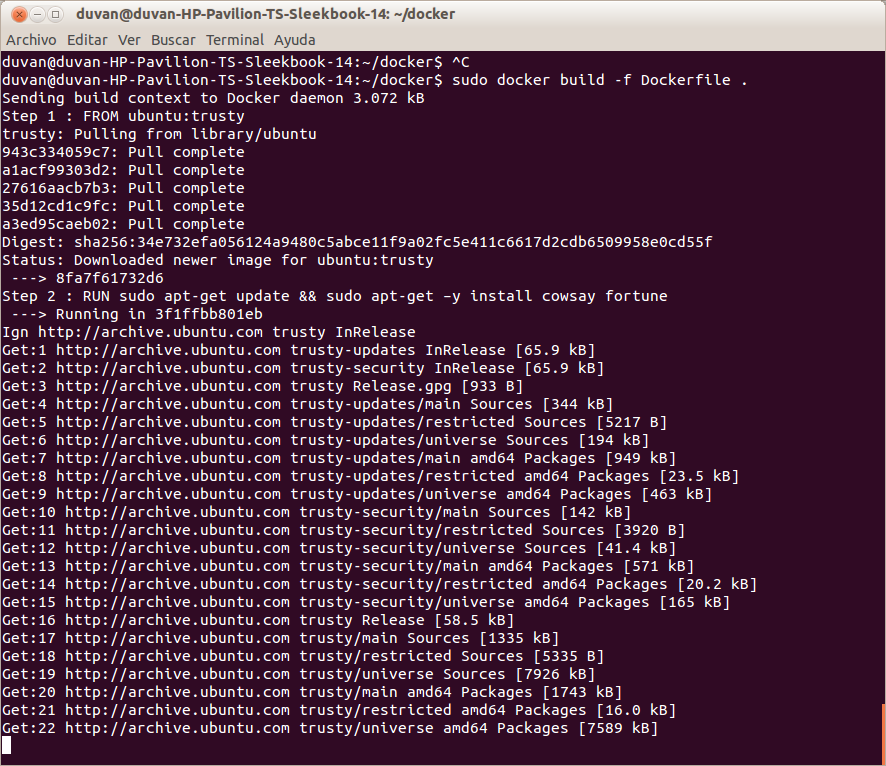
\includegraphics[scale=0.35]{4}   
	\caption{Construcción de la imagen} 
\end{figure}

\begin{figure}[ht]
	\centering
	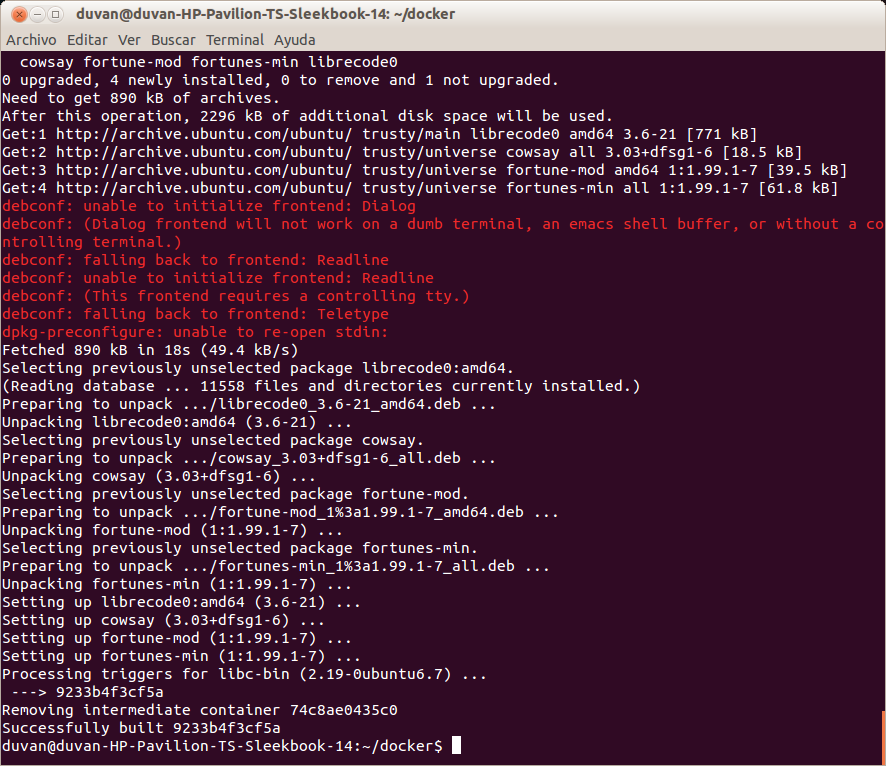
\includegraphics[scale=0.4]{41}   
	\caption{Construcción de la imagen} 
\end{figure}

\item Ejecutar un nuevo contenedor a partir de la imagen creada.

\begin{center}
	\texttt{sudo docker run test/dockerfile-example /usr/games/cowsay “Hola a todos!”}
\end{center}
\begin{figure}[ht]
	\centering
	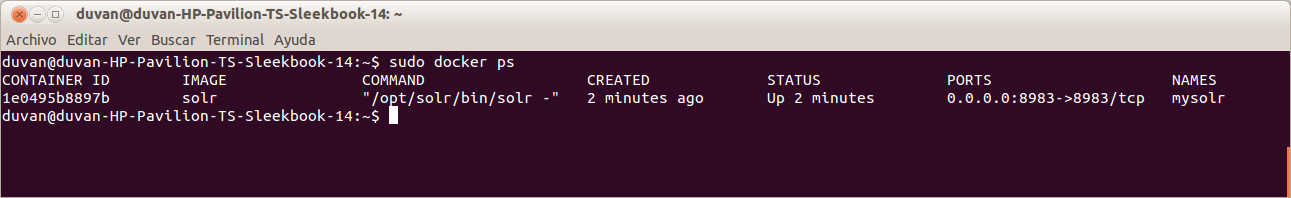
\includegraphics[scale=0.35]{5}   
	\caption{Ejecución de un nuevo contenedor} 
\end{figure}
\begin{figure}[H]
	\centering
	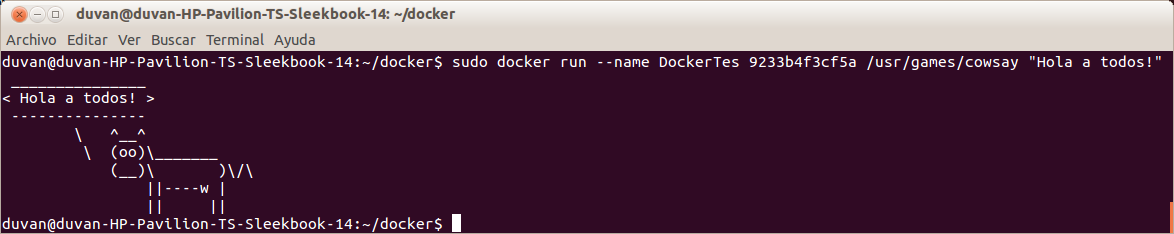
\includegraphics[scale=0.35]{51}   
	\caption{Ejecución de un nuevo contenedor} 
\end{figure}

\end{enumerate}

\section{BIBLIOGRAFÍA}

\begin{itemize}
	\item \href{https://www.docker.com/what-docker}{https://www.docker.com/what-docker}
	
	
\end{itemize}
	
\end{document}
